\documentclass[a4paper, notitlepage, 10pt]{article}
\usepackage{geometry}
% WSC 2015 configs
\fontfamily{times}
\geometry{verbose,tmargin=30mm,bmargin=25mm,lmargin=25mm,rmargin=25mm}
\pagestyle{empty}
% end configs
\usepackage{setspace,relsize}               
\usepackage{moreverb}                        
\usepackage{url}
\usepackage{hyperref}
\hypersetup{colorlinks=true,citecolor=blue}
\usepackage{amsmath}
\usepackage{mathtools} 
\usepackage{amsthm}
\usepackage{amssymb}
\usepackage{indentfirst}
\usepackage{todonotes}
\usepackage[authoryear,round]{natbib}
\bibliographystyle{apalike}
\usepackage[pdftex]{lscape}
\usepackage[utf8]{inputenc}
% Title Page
\title{\vspace{-9ex}\centering \bf On the choice of the weights for the logarithmic pooling of probability distributions}
\author{
Luiz Max F. de Carvalho$^{a,b,c}$, Daniel A. M. Villela$^a$, Flavio Coelho$^c$ \& Leonardo S. Bastos$^a$ \\
a -- Program for Scientific Computing (PROCC), Oswaldo Cruz Foundation. \\
b -- Institute of Evolutionary Biology, University of Edinburgh.\\
c -- School of Applied Mathematics, Getulio Vargas Foundation (FGV).
}
\DeclareMathOperator*{\argmin}{arg\,min}
\DeclareMathOperator*{\argmax}{arg\,max}
\newtheorem{theo}{Theorem}[]
\newtheorem{proposition}{Proposition}[]
\newtheorem{remark}{Remark}[]
\setcounter{theo}{0} % assign desired value to theorem counter
\begin{document}
\maketitle

\begin{abstract}
Combining different prior distributions is an important issue in decision theory and Bayesian inference.
Logarithmic pooling is a popular method to aggregate expert opinions by using a set of weights that reflect the reliability of each information source.
The resulting pooled distribution however heavily depends set of weights given to each opinion/prior.
In this paper we explore three approaches to assigning weights to opinions.
Two methods are stated in terms of optimisation problems and a third one uses a hierarchical prior that accounts for uncertainty on the weights. 
We explore several examples of interest, such as proportion and rate estimation and combining Normal distributions.
Our findings...

Key-words: logarithmic pooling; expert opinion; maximum entropy; Kullback-Leibler divergence; Dirichlet prior. 
\end{abstract}

\section*{Introduction}

Combining probability distributions is a topic of general interest, both in the statistical~\citep{west1984, genest1986A, genest1986B} and decision theory literatures~\citep{genest1984}.
On the theoretical front, studying opinion pooling operators may give important insights on consensus belief formation and group decision making~\citep{genest1986B}.
Among the various opinion pooling operators proposed in the literature, logarithmic pooling has enjoyed much popularity, mainly due to its many desirable properties such as relative propensity consistency (RPC) and external Bayesianity (EB)~\citep{genest1986A}. 
In a practical setting, logarithmic pooling finds use in a range of fields, from infectious disease modelling~\citep{Coelho2009} and wildlife conservation~\citep{poole2000} to engineering~\citep{lind1988, savchuk1994}.

A common situation of interest is that of combining expert opinions, represented as proper probability distributions, about a quantity of interest $\theta \in \mathbf{\Theta} \subseteq \mathbb{R}^p$.
To combine these opinions using logarithmic pooling requires assigning weights to each of the experts.
These weights represent the reliability of each opinion~\citep{genest1984}.
This requirement naturally leads to the question of how to choose the weights in a meaningful fashion, according to some well-accepted optimality criterion.
There are a few proposals in the literature that build methods using different approaches.
One proposal is to maximise the entropy the pooled distribution~\citep{myung1996}, whereas another one is to minimise Kullback-Leibler (KL) divergence between the pooled distribution and the individual opinions~\citep{abbas2009} or between the pooled (prior) distribution and the posterior distribution~\citep{rufo2012A,rufo2012B}.

These approaches, while moving away from the problem of arbitrarily assigning the weights, arrive at single point solutions, similar to point estimates in Statistical theory.
Albeit acknowledging that these approaches have merit, we argue that in many settings, where one has substantial prior information on the relative reliabilities of the information sources (experts), it would be desirable to incorporate this information into the pooling procedure while accommodating uncertainty about the weights~\citep{poole2000}.
Moreover, assigning a probability distribution over the weights allows one to obtain a posterior distribution using a Bayesian procedure, which in turn enables learning about the weights from data.
Therefore, it makes possible to sequentially update knowledge about the reliability of each expert/source in the face of new data.


DEFINE MSM, MELDING. 


In this paper we explore previous approaches for deriving the weights for logarithmic pooling, namely by maximising the entropy of the resulting distribution and minimising the KL divergence between the pooled distribution and each individual distribution.
Additionally, we propose a hierarchical prior approach in which we place a distribution on the weights.
We also discuss the case where the decision maker is interested in a transformation $y$ of the quantity $\theta$ for which the expert opinions were elicited.
To conclude, we present three examples in different contexts illustrating the choice of weights for the logarithmic pooling. %an example on proportion estimation by combining Beta priors.
In the first example we combine some distributions of the prevalence of the human immunodeficiency virus (HIV) in man who have sex with another man (MSM) extracted from a meta analysis study.
The second example we apply the log-pooling operator by combining elicited Beta priors... [Simple description here]
Finally, the third example we revisit the Bayesian melding model... [Simple description here]

\section*{Background}

%\section*{Properties of the logarithmic pooling operator}

In what follows, we introduce the necessary theory and notation and motivate the use of the logarithmic pooling operator by presenting some of its desirable properties.

First let us define the logarithmic pooling (LP) operator.
Let $\mathbf{F}_{\theta} := \{f_0(\theta), f_1(\theta), f_2(\theta), \ldots, f_K(\theta)\}$ be a set of prior distributions representing the opinions of $K+1$ experts and let $\boldsymbol\alpha :=\{\alpha_0, \alpha_1, \alpha_2, \ldots, \alpha_K \}$ be the vector of weights, such that $\alpha_i > 0\: \forall i$ and $\sum_{i=0}^K \alpha_i = 1$.
Then the log-pooled prior is
\begin{equation}
\label{eq:logpool}
 \mathcal{LP}(\mathbf{F_\theta}, \boldsymbol\alpha) := \pi(\theta) = t(\boldsymbol\alpha) \prod_{i=0}^K f_i(\theta)^{\alpha_i},
\end{equation}
where $t(\boldsymbol\alpha) = \int_{\boldsymbol\Theta}\prod_{i=0}^K f_i(\theta)^{\alpha_i}d\theta$.

Logarithmic pooling will only yield proper probability distributions if it is possible to normalise the expression in (\ref{eq:logpool}).
% This condition is usually assumed implicitly, without proof.
While \citet{poole2000} provide a proof for the case of two densities (see Theorem 1 therein),~\cite{genest1986A} (pg.489) prove the result for a finite number of densities.
\begin{theo}
\label{thm:normalisation}
\textbf{Normalisation~\citep{genest1986A}}. 
Let $A$ be a $(K+1)$-dimensional open simplex on $[0,1]$.
For all $\boldsymbol\alpha \in A$ there exists a constant $t(\boldsymbol\alpha)$ such that $\int_{\boldsymbol\Theta}\pi(\theta)d\theta = 1$.
\end{theo}
A simple proof using H\"{o}lder's inequality is given in the Appendix of this paper.
This result ensures any (finite) number of proper distributions can be combined using the logarithmic pooling operator to yield a normalisable (proper) density.

Another interesting property of the logarithmic pooling operator is the fact that combining log-concave densities will produce a log-concave pooled distribution.
\begin{remark}
\label{rmk:concavity}
\textbf{Log-concavity}. 
 Let $\mathbf{F}_{\theta}$ be a set of log-concave distributions, i.e., each $f_i$ can be represented as $ f_i(\theta) \propto e^{\psi_i(\theta)}$,
%  \begin{equation}
%   \label{eq:logconcavity}
%   f_i(\theta) \propto e^{\psi_i(\theta)},
%  \end{equation}
where $\psi_i(\cdot)$ is a concave function.
Then $\pi(\theta)$ is also log-concave.
\end{remark}

Log-concavity of the pooled prior may be important to consider in order to guarantee unimodality and certain conditions on tail behaviour.



\subsection*{Exponential family}

Suppose we are interested in a random variable, $Y$, from a exponential family with parameter $\theta$ and probability density function given by
\begin{equation}
\label{eq:exponentialfamily}
f(y|\theta) = h(y) e^{\theta y - s(\theta)}.
\end{equation}

Let $\mathbf{F}_{y}$ be a set of distributions on $y$ of the form in~(\ref{eq:exponentialfamily}), $f_i(y|\theta_i)$, $ i = 0, 1, \ldots, K$. 
The combined (log-pooled) distribution also belongs to the exponential family:

\begin{equation}
\label{eq:pooldistEF}
\pi(y| \boldsymbol\alpha ) = t(\boldsymbol\alpha) h^\ast (y) e^{\theta^\ast y - s^\ast (\boldsymbol\theta)}.
\end{equation}
where $\boldsymbol\theta :=\{\theta_0, \theta_1, \ldots, \theta_K \}$, $h^\ast (y) = \prod_{i = 0}^K h_i(y)^{\alpha_i}$,  $\theta^\ast = \sum_{i = 0}^K \alpha_i \theta_i$ and $s^\ast (\boldsymbol\theta) = \sum_{i = 0}^K \alpha_i s_i(\theta_i)$.

The entropy function of the log-pooled distribution is
\begin{equation}
\label{eq:entropydistEF}
H_\pi(Y; \boldsymbol\alpha) :=  - E_{\pi}\left[-\log \pi(Y | \boldsymbol\alpha) \right] = -\log t(\boldsymbol\alpha) + s^\ast (\boldsymbol\theta) - \mathbb{E}_\pi[\log h^\ast (Y)] - \theta^\ast \mathbb{E}_\pi[Y] \: ,
\end{equation}
and the Kullback-Leibler divergence between the pooled distribution (\ref{eq:pooldistEF}) and each distribution in $\mathbf{F}_{y}$ can be written as:
\begin{equation}
\label{eq:KLdistEF}
KL(\pi || f_i )  =  - H_\pi(Y; \boldsymbol\alpha) - \mathbb{E}_\pi[\log h_i(Y)] - \theta_i \mathbb{E}_\pi[Y] + s_i(\theta_i) \: .
\end{equation}

These expressions allow for easy computation of information measures for a broad class of distributions, which will be useful in the remainder of this paper.

\subsection*{Conjugate priors for exponential family}

A conjugate prior family for $f(y|\theta)$, given in (\ref{eq:exponentialfamily}), is the following
\begin{equation}
\label{eq:priorEF}
g(\theta | a, b) = K(a,b) e^{\theta a - b s(\theta)} \: ,
\end{equation}
where $K(a,b)$ is a normalising constant.
Here, we employ the definition and notation for exponential family and its conjugate prior family from \citet[chapter 3]{robert2001}. % with an exception for the \psi function, which is used for the digamma function later on.
Similar to the above, let $\mathbf{G}_{\theta}$ be a set of conjugate prior distributions representing the opinions of $K+1$ experts, and $g_i(\theta) = g(\theta | a_i, b_i)$ from equation (\ref{eq:priorEF}).

The log-pooled prior is also a conjugate prior for $f(y|\theta)$ with hyperparameters given by an weighted mean of the experts hyperparameters, i.e., $\pi(\theta|\boldsymbol\alpha) = g(\theta | a^*, b^* )$, where $a^* = \sum_{i=0}^K \alpha_i a_i$ and $b^* = \sum_{i=0}^K \alpha_i b_i$.
% \begin{equation}
% \label{eq:poolpriorEF}
% \pi(\theta|\boldsymbol\alpha) = g(\theta | a^*, b^*) \: ,
% \end{equation}
% where $a^* = \sum_{i} \alpha_i a_i$ and $b^* = \sum_{i} \alpha_i b_i$.
% Note that the posterior distribution of $\theta$ is given by $\pi(\theta | y) = g(\theta | a^* + y, b^* + 1)$.

The entropy function of the log-pooled prior (\ref{eq:priorEF}) is given by
\begin{equation}
\label{eq:entropypriorEF}
H_\pi(\theta; \boldsymbol\alpha) = - \log (K(a^*, b^*))  -  a^*  \mathbb{E}_\pi[\theta]  +  b^*  \mathbb{E}_\pi[s(\theta)] \: .
\end{equation}

And the Kullback-Leibler divergence, $KL(\pi || g_i )$, is the following
\begin{equation}
\label{eq:KLpriorEF}
KL( \pi || g_i ) = - H_\pi(\theta; \boldsymbol\alpha) - \log( K(a_i,b_i)) - a_i \mathbb{E}_\pi[\theta] + b_i \mathbb{E}_\pi[s(\theta)] \: .
\end{equation}

We now move on to study three approaches to assign weights.
The first two approaches are based on optimality criteria and a third method is based on assigning a Dirichlet hyperprior on the weights.


\section*{Assigning the weights in logarithmic pooling}

\subsubsection*{Choosing the weights by maximising entropy}

In a context of near complete uncertainty about the relative reliabilities of the experts (information sources) it may be desirable to combine the prior distributions such that $\pi(\theta)$ is maximally uninformative. %% LM: this can be highly problematic...
Such approach would ensure that, given the constraints imposed by $\mathbf{F}_{\theta}$, the pooled distribution is the one which best represents the current state of knowledge~\citep{jaynes1957,savchuk1994}.
In order to choose $\boldsymbol\alpha$ so as to maximise prior 
diffuseness, one can maximise the entropy of the log-pooled prior.  
%
%i.e.:
%\begin{equation}
%\label{eq:entropypiA}
%H_{\pi}(\theta) = E_{\pi}\left[-\log \pi(\theta) \right] =-\int_{\boldsymbol\Theta}\pi(\theta)\ln\pi(\theta)d\theta 
%\end{equation}
%
%In some cases it may be useful to express $H_{\pi}(\theta)$ as
%\begin{equation}
%\label{eq:entropypiB}
% H_{\pi}(\theta; \boldsymbol\alpha) = \sum_{i=0}^{K} \alpha_i E_{\pi}[ - \ln f_i(\theta)] - \ln t(\boldsymbol\alpha)
%\end{equation}
Formally, we want to find $\hat{\boldsymbol\alpha}$ such that
\begin{equation}
\label{eq:argmaxEnt}
 \hat{\boldsymbol\alpha}:= \argmax H_{\pi}(\theta; \boldsymbol\alpha).
\end{equation}

This approach, however, does not result in a convex optimisation problem, therefore one is not guaranteed to find a unique solution. 
See Proposition~\ref{remark:uniqueness}, below, for intuition as to why.

\subsubsection*{Choosing the weights by minimising Kullback-Leibler divergence}

One could also want to choose the pooling weights so as to minimise the total Kullback-Leibler divergence between the pooled distribution, $\pi$, each proposed distribution in $\mathbf{F}_{\theta}$.
Let $d_i = \text{KL}(\pi || f_i)$ and let $L(\boldsymbol\alpha)$ be a loss function such that
\begin{align}
L(\boldsymbol\alpha) &= \sum_{i=0}^K d_i \\
\label{eq:KLexpanded}
     &= - (K+1) H_\pi(\theta; \boldsymbol\alpha)  - \sum_{i=0}^K \mathbb{E}_\pi\left[\log f_i(\theta) \right] \\
     \label{eq:argminKL}
     \hat{\boldsymbol\alpha}:=& \:\argmin L(\boldsymbol\alpha)   
\end{align}

[DO WE NEED UNIQUENESS?]

\begin{remark}
\label{remark:uniqueness}
\textbf{Uniqueness}~\citep{rufo2012A}.
 The distribution obtained following~(\ref{eq:argminKL}) is unique, i.e., there is only one aggregated prior $\pi(\theta)$ that minimizes $L(\boldsymbol\alpha)$.
\end{remark}
One can get some intuition into the proof  of this claim by noting that minimising~(\ref{eq:KLexpanded}) is equivalent to maximising $\ln t(\boldsymbol\alpha) = \ln\int_{\boldsymbol\Theta}\prod_{i=0}^{K}f_i(\theta)^{\alpha_i}d\theta$. 
\cite{rufo2012A} show that $t(\boldsymbol\alpha)$ is concave, therefore the problem in~(\ref{eq:argminKL}) has a unique solution.
By contrast, the problem in~(\ref{eq:argmaxEnt}) requires to minimise $\ln t(\boldsymbol\alpha)$ hence lacking a sufficient condition for the existence of a unique solution.



\subsubsection*{Minimising Kullback-Leibler divergence in transformed space}

[IS THIS IMPORTANT?]

One might argue that procedure (b) makes little sense, given that the set of opinions $\mathbf{F}_{\theta}$ concerns only $\theta$, i.e, it was not necessarily constructed taking the transformation $M(\cdot)$ into account.
An example is a situation where experts are asked to provide distributions on the probability $p$ of a particular event.
In general, elicitation for $f_i(p)$ will not take into account the induced distribution on the log-odds, $M(p) = \log p/(1-p)$.
%% LM: we can change this dull example to something more involved.
Nevertheless, the decision-maker may wish to assign the weights $\boldsymbol\alpha$ in a way that takes $M(\cdot)$ into account, e.g., by giving lower weights to experts whose distributions on the log-odds scale are unreasonable.

This decision process can be made more precise.
In a similar spirit to the discussed above, one can construct $\boldsymbol\alpha$ so as to minimise the Kullback-Leibler divergence between each distribution in $\mathbf{F^{-1}_y}$ and a transformation of the distribution obtained by procedure (a), $\pi_{y}(y | \boldsymbol\alpha) = \pi_{\theta}( M^{-1}(y)| \boldsymbol\alpha)|J|$.
Let $d_i = \text{KL}( h_i(y) || \pi_{y}(y | \boldsymbol\alpha))$.
We then aim at solving the problem
\begin{align}
L(\boldsymbol\alpha) &= \sum_{i=0}^Kd_i \\
     \hat{\boldsymbol\alpha}:=& \:\argmin L(\boldsymbol\alpha)  \nonumber
\end{align}

This procedure therefore choses weights for each expert by how coherent the prior provided by each expert is with the pool-then-induce -- procedure (a) -- prior in the transformed space induced by $M(\cdot)$.

\subsection*{Hierarchical modelling of the weights}

In this section we propose assigning prior distributions for the weights.

A natural choice for a prior distribution for $\boldsymbol\alpha$ is the $(K+1)-$dimensional Dirichlet distribution.
\begin{equation}
 \label{eq:generalcondprior}
 \pi(\boldsymbol\alpha) = \frac{1}{\mathcal{B}(\boldsymbol x)}\prod_{i=0}^K \alpha_i^{x_i-1}
\end{equation}
where $\boldsymbol x = \{ x_0, x_1, \ldots, x_K\}$ is the vector of hyperparameters for the Dirichlet prior and $\mathcal{B}(X)$ is the multinomial beta function.
The marginal prior for $\theta$ is then
\begin{align}
 \label{eq:marginalhierprior}
 \pi(\theta) &= \int_{A}\pi(\theta|\boldsymbol\alpha)\pi(\boldsymbol\alpha)d\boldsymbol\alpha \\
             &= \frac{1}{\mathcal{B}(\boldsymbol x)}\int_{A}t(\boldsymbol\alpha)\prod_{i=0}^K f_i(\theta)^{\alpha_i}\alpha_i^{x_i-1}d\boldsymbol\alpha 
\end{align}


A more flexible prior for $\boldsymbol\alpha$ is the logistic-normal distribution~\citep{aitchson1980}. 
\begin{equation}
 \label{eq:aitchinsonprior}
 \pi(\boldsymbol\alpha) = \frac{1}{|2\pi \boldsymbol \Sigma|^{\frac{1}{2}}}\frac{1}{\prod_{i=0}^K \alpha_i}
  e^{
     \left(\log\left(\frac{\boldsymbol \alpha_{-K}}{\alpha_K}\right) - \boldsymbol \mu\right)^T
     {\boldsymbol \Sigma}^{-1}
     \left(\log\left(\frac{\boldsymbol \alpha_{-K}}{\alpha_K}\right) - \boldsymbol \mu\right)
     }
\end{equation}
where $\boldsymbol \alpha_{-K}$ represents the vector $\boldsymbol \alpha$ without the $K$-th element, $\boldsymbol \mu$ is a $K$-size mean vector, and $\boldsymbol \Sigma$ is a $K \times K$ covariance matrix. \citet{aitchson1980} propose choosing $\boldsymbol \mu$ and $\boldsymbol \Sigma$ minimizing the KL divergence between the Dirichlet (\ref{eq:generalcondprior}) and the logistic-normal (\ref{eq:aitchinsonprior}) distributions, i.e.
\begin{align}
 \label{eq:momentmatching}
 \mu_i & = \psi(x_i) - \psi(x_K), \quad i=0,1,\ldots,K-1, \\
 \Sigma_{ii} & = \psi'(x_i) + \psi'(x_K), \quad i=0,1,\ldots,K-1, \\
 \Sigma_{ij} & = \psi'(x_K)
\end{align}
where $\psi(\cdot)$ is the digamma function, and $\psi'(\cdot)$ is the trigamma function.



%a hierarchical prior for $\theta$ conditional on $\boldsymbol\alpha$ in order to incorporate uncertainty on the weights.
%The conditional distribution $\pi(\theta|\boldsymbol\alpha)$ is of the form in~(\ref{eq:logpool}) and the prior density for $\boldsymbol\alpha$ is 
%\subsubsection*{Priors}
%
%\subsubsection*{Posterior}
%\begin{align}
% \label{eq:alpha_posterior}
% p(\boldsymbol\alpha | x) &= \int_{\Theta}  p(\theta, \boldsymbol\alpha | x) d\theta \\
%  &\propto  \int_{\Theta} \mathcal{L}(x | \theta) \pi(\theta | \boldsymbol\alpha) \pi(\boldsymbol\alpha) d\theta
%\end{align}
%
%\subsubsection*{Computational approach}

\section*{Applications}

\label{sec:apps}

\subsection*{HIV prevalence among MSM populations in Brazil}

In epidemiology, systematic review and meta analysis are popular tools for merging and contrasting results across multiple studies \citep[Chapter 33]{Rothman2008}. 
For instance, the logarithmic polling could be used to combine probability distributions of a particular outcome estimated from several studies. 
We illustrate the different approaches to assign weights in the logarithmic polling in the systematic review and meta analysis conducted by \citet{malta2010hiv}. 
They analysed studies published from 1999 to 2009 assessing the HIV prevalence among men who have sex with another men (MSM) in Brazil. 
The authors have found six studies that estimated HIV prevalence in MSM population in Brazil. 

Assuming a uniform prior for the HIV prevalence among MSM, denoted by $\theta$, and a binomial model for each study, i.e. $Y_i \sim Binom(n_i, \theta)$. 
The posterior distribution for the HIV prevalence conditional on each study is then a Beta distribution with parameters $a_i = y_i + 1$ and $b_i = n_i - y_i + 1$, for $i=0,1,2,3,4,5$. 
The probability density of the HIV prevalence for each study is given by
$$f_i(\theta;a_i, b_i) = \frac{1}{B(a_i b_i)} \theta^{a_i-1}(1-\theta)^{b_i-1},$$
where $B(a,b) := \int_{0}^{1} x^{a-1}(1-x)^{b-1}dx$ is the Beta function.

Table \ref{tbl:hivmsm} presents for each study the sample size, the total of HIV positive observed, and the estimated prevalence given by the expectation of the Beta distribution with 95\% credible interval. 
Note that the estimated prevalences among MSM are very high when compared with the HIV prevalence in the general population, 0.6\% \citep{malta2010hiv}.
\begin{table}[ht]
\caption{Data extracted from the systematic review and meta analysis conducted by \citet{malta2010hiv} assessing the HIV prevalence among MSM in Brazil. $n$ is the sample size, $y$ is the total of HIV-positive participants. }
\label{tbl:hivmsm}
\centering
\begin{tabular}{rlrrr}
  \hline
Study & Reference & $n$ & $y$ & Estimated prevalence (95\% CI)\\ 
  \hline
0 & \cite{tun2008sexual}            &  658 &  44 & 0.0682  (0.0502, 0.0886) \\ 
1 & \cite{barcellos2003prevalence}  &  461 & 111 & 0.2419  (0.2040, 0.2819) \\ 
2 & \cite{carneiro2003determinants} &  621 &  61 & 0.0995  (0.0773, 0.1242) \\ 
3 & \cite{sutmoller2002human}       & 1165 & 281 & 0.2416  (0.2175, 0.2666) \\ 
4 & \cite{BMH2000}                  &  642 &  57 & 0.0901  (0.0692, 0.1133) \\ 
5 & \cite{harrison1999incident}     &  849 &  99 & 0.1175  (0.0968, 0.1400) \\ 
   \hline
\end{tabular}
\end{table}


The log-pooled distribution for the HIV prevalence is then
\begin{align}
\pi(\theta) & = t(\boldsymbol\alpha)\prod_{i=0}^{K}f_i(\theta;a_i,b_i)^{\alpha_i}\\
            & \propto \prod_{i=0}^{K} \left(\theta^{a_i-1}(1-\theta)^{b_i-1} \right)^{\alpha_i}\\
\label{eq:betabern}
&\propto \theta^{a^*-1}(1-\theta)^{b^*-1}
\end{align}
with $a^* =\sum_{i=0}^{K}\alpha_ia_i$ and $b^* = \sum_{i=0}^{K}\alpha_ib_i$.
Note that (\ref{eq:betabern}) is the kernel of a Beta distribution with parameters $a^*$ and $b^*$. Hence the entropy is the following
\begin{equation}
 \label{eq:entropybeta}
 H_{\pi}(\theta) = \log B(a^*,b^*) - (a^*-1)\psi(a^*) - (b^*-1)\psi(b^*) + (a^*+b^* -2)\psi(a^*+b^*).
\end{equation}
And the KL divergence between $\pi(\theta)$ and $f_i(\theta)$  is
\begin{equation}
\begin{split}
 \label{eq:KLbeta}
 d_i = KL(\pi || f_i) = \ln\left(\frac{\mathcal{B}(a_i, b_i)}{\mathcal{B}(a^*, 
b^*)}\right) & + (a^* - a_i) \psi(a^*)+ (b^* - b_i)\psi(b^*) \\
 &- (a^*-a_i + b^* - b_i)\psi(a^*+b^*).
\end{split}
 \end{equation}

Table \ref{tab:probMeta} shows the estimates of the HIV prevalence among MSM in Brazil using different methods of dealing with weights. 
The first method assumes all studies are equally important, i.e. $\alpha_i = \frac{1}{K}, \quad \forall i$. The second method maximizes the entropy given in (\ref{eq:entropybeta}) which in this example corresponds to $(\alpha_3 = 1, \alpha_j = 0 \quad \forall j \neq 3)$. 
This method gave all the weight for the study 3 by \cite{sutmoller2002human} which is the study with the larger sample size. 
The remaining methods, minimizing the KL divergence and the hierarchical modelling of weights suggest that all studies should have the same weight, however in the hierarchical approach the weights probability distribution is numerically integrated out leading to larger 95\% credible intervals. 
\begin{table}[ht]
\caption{Estimated HIV prevalence (95\% credible interval) among men who have sex with another man in Brazil using different methods for assessing the weights.}
\centering
\label{tab:probMeta}
\begin{tabular}{cc}
 \hline
Method & Estimated HIV prevalence \\ 
 \hline
 Equal weights                & 0.1495   (   0.1247  ,    0.1762) \\ 
 Maximum entropy              & 0.2416   (   0.2175  ,    0.2666) \\ 
 Minimum KL                   & 0.1495   (   0.1247  ,    0.1762) \\ 
 Hierarchical Dirichlet prior & 0.1478   (   0.0941  ,    0.2117) \\ 
 Hierarchical Aitchison prior & 0.1471   (   0.0878  ,    0.2245) \\ 
  \hline
\end{tabular}
\end{table}




\subsection*{Combining expert priors on failure probabilities [MELHORAR]}
\label{sec:beta}

We now turn our attention to combining expert opinions about probabilities and proportions.
%In this setting we are interested in the random variable $Y | \theta \sim Bernoulli(\theta)$.
%Assume that we want to obtain a combined prior for a proportion $\theta$.
Here we analyse an example proposed by~\cite{savchuk1994} (also discussed in~\cite{rufo2012B}) in which four experts are required supply prior information about the survival probability of a certain unit, $\theta$, for which there have been $y = 9$ successes out of $n = 10$ trials.
The experts express their opinion as prior means for the survival probability, which~\cite{savchuk1994} then use to construct prior distributions with maximum variance given the restriction on the means.
From the vector of prior means $\mathbf{m} = \{ m_0 = 0.95, m_1 = 0.80, m_2 = 0.90, m_3 = 0.70 \}$, the authors obtain the parameters of the beta distributions for each expert,  $\mathbf{a} = \{ a_0 = 18.10, a_1 = 3.44 , a_2 = 8.32, a_3 = 1.98 \}$ and  $\mathbf{b} = \{ b_0 = 0.955 , b_1 = 0.860, b_2 = 0.924, b_3 = 0.848\}$.
Note that this example is quite similar to the previous one in the sense that the aim is to combine beta distributions. 
However, we are able to estimate the posterior distribution for the surviving probabilities and also, in the hierarchical modelling approach, the posterior distribution for the weights.

Table~\ref{tab:alphasBeta} lists the weights proposed by each method.
Figure~\ref{fig:priors_posteriors_beta} shows the prior and posterior distributions in each of the methods and also the case in which we assign an equal weight ($1/K$) to each opinion.
It is interesting to note that maximum entropy suggests to discard all opinions but one, which effectively leads to the maximum entropy.
Since $t(\boldsymbol\alpha)$ is concave, we expect to find the maximum entropy given by the boundary conditions, which may lead to border points in the simplex.
Minimising Kullback-Leibler divergence between each prior and the pooled prior leads to finding a unique solution but in this case also suggests to discard two of the opinions. [NEEDS UPDATE!]
By contrast, using a hierarchical Dirichlet prior for the weights gives rather different results from the first two methods in proposing almost equal weights to each of the opinions.

\begin{table}[ht]
\caption{Weights obtained using the three methods for the proportion estimation problem. $^1$ -- Kullback-Leibler $^2$ -- Posterior mean for $\boldsymbol\alpha$.}
\centering
\begin{tabular}{ccccc}
  \hline
Method  & $\alpha_0$ & $\alpha_1$ & $\alpha_2$ & $\alpha_3$ \\ 
  \hline
Maximum entropy & 0.00 & 1.00 & 0.00 & 0.00 \\ 
Minimum KL$^1$ divergence& 0.04 & 0.96 & 0.00 & 0.00 \\ 
Hierarchical prior$^2$ & 0.26 & 0.24 & 0.26 & 0.23 \\ 
   \hline
\end{tabular}
\label{tab:alphasBeta}
\end{table}

%The marginal prior for $\theta$ is
%\begin{equation}
%\label{eq:marginalbeta}
%\pi(\theta) = \frac{1}{\mathcal{B}(X)}\int_{A} \frac{1}{\mathcal{B}(a^*, b^*)} \theta^{a^* -1}(1-\theta)^{b^* -1}\alpha_i^{x_i-1}d\boldsymbol\alpha 
%\end{equation}
%which can also be efficiently approximated through Monte Carlo sampling.
%We provide a simple implementation using the Stan~\citep{stan2014} probabilistic programming language at~\url{https://github.com/maxbiostat/opinion_pooling}.
%R code for the methods, figures and tables presented in this paper can also be found at the above link.

%The resulting prior densities are show in the top panel of Figure~\ref{fig:priors_posteriors_beta}.
To complete the analysis, we place a diffuse $Dirichlet(\boldsymbol\alpha | \boldsymbol X)$ prior on $\boldsymbol\alpha$ with $X_i = 1/4 \: \forall i$.
Finally, we propose to compare the prior distributions representing the experts' opinions as well as the combined distributions obtained by the different approaches using the integrated (marginal) likelihood (\cite{raftery2007}, eq. 9), $l(y) = \int_{0}^{1}f(y|\theta)\pi(\theta)d\theta$.
The marginal likelihood for the $i-th$ expert and $J$ observations of the form $\{ y_j, n_j\}$ is:
\begin{align}
  \label{eq:marglike}
l_i(y_j) &= \int_{0}^{1}\mathcal{L}(\theta|y_j, n_j)\pi_i(\theta)d\theta\nonumber\\
 &= \prod_{j = 1}^{J}\frac{\Gamma(n_j-1)}{\Gamma(n_j-y_j + 1)\Gamma(y_j+1)}\frac{\Gamma(a_i + b_i)}{\Gamma(a_i + b_i + n_j)}\frac{\Gamma(a_i + y_j)}{\Gamma(a_i)}\frac{\Gamma(b_i + n_j - y_j) }{\Gamma(b_i)}
 \end{align}


One can get insight into these results by looking at the integrated likelihoods in Table~\ref{tab:marglikes} and the densities in Figure~\ref{fig:priors_posteriors_beta}, we note that all three methods lead  to similar pooled distributions.
Note that the only distribution with a substantially different $l(y)$ is that of Expert 3, who gave a rather divergent mean for the survival probability ($m_3=0.70$).

\begin{table}[ht]
\caption{Integrated likelihoods ($l(y)$) for the priors of each expert as well as the combined priors.
$^1$ Calculated using the posterior mean of $\boldsymbol\alpha$}
\centering
\begin{tabular}{cccc}
   \hline
   \multicolumn{2}{c}{Expert priors} &  \multicolumn{2}{c}{Pooled priors} \\
   \hline
   Expert 0 & 0.237 & Equal weights & 0.254\\
   Expert 1 & 0.211 & Maximum entropy & 0.211 \\
   Expert 2 & 0.256 & Minimum KL & 0.223\\ 
   Expert 3 & 0.163 & Hierarchical$^1$ & 0.255 \\
   \hline
\end{tabular}
\label{tab:marglikes}
\end{table}
%%%%%%%%%%%%%%%%%%

In conclusion, if the prior distributions (opinions) are not radically different, all three methods will probably lead to similar combined priors.
Although this is the case for the simple univariate example presented, it remains to be seen if this is the case for high-dimensional $\theta$ under complex sampling distributions.
As the results presented in this paper make clear, future research shall be focused on cases where there is substantial heterogeinity in the available opinions.
Moreover, a sensitivity analysis for $\pi(\boldsymbol\alpha)$ is desirable to understand how much we can lead about the experts reliabilities~\textit{a posteriori}.



\begin{table}[ht]
\centering
\begin{tabular}{ccc}
 \hline
Method & Prior & Posterior  \\ 
 \hline
 Equal weights & 0.90 (0.64--1.00) & 0.90 (0.73--0.99) \\ 
 Maximum entropy & 0.80 (0.37--1.00) & 0.87 (0.66--0.98) \\ 
 Minimum KL  & 0.82 (0.42--1.00) & 0.87 (0.67--0.99) \\ 
 Hierarchical Dirichlet prior & 0.88 (0.53--1.00) & 0.90 (0.71--0.99) \\ 
 Hierarchical Aitchinson prior & ? (?--?) & ? (?--?) \\ 
  \hline
\end{tabular}
\label{tab:prior_posteriorsBeta}
\end{table}
%%%%%%%%%%%%%%%%%%%%


% Results run from Leo's laptop (rstan needs to be updated, hence no posterior for hierarchical modelling)

%> AlphasBeta.tbl
%                 alpha0       alpha1       alpha2       alpha3
%maxEnt             1.00 2.527039e-20 1.550258e-14 4.644285e-12
%min KL div.        0.25 2.500000e-01 2.500000e-01 2.500000e-01
%Hier. prior Diri     NA           NA           NA           NA
%Hier prior Exp       NA           NA           NA           NA


%> PaperBeta.tbl
%                 mean.prior lower.prior upper.prior mean.post lower.post
%Equal weights     0.8977359   0.6435035   0.9979079 0.8989360  0.7327552
%maxEnt            0.9478921   0.8160731   0.9986309 0.9314315  0.8173654
%min KL div.       0.8977359   0.6435035   0.9979079 0.8989360  0.7327552
%Hier. Diri  0.8787021   0.5265047   0.9978187        NA         NA
%Hier Exp    0.8725528   0.4803808   0.9977648        NA         NA
%                 upper.post
%Equal weights     0.9877894
%maxEnt            0.9913162
%min KL div.       0.9877894
%Hier. prior Diri         NA
%Hier prior Exp           NA

%\subsubsection*{Simulated data}

\subsection*{Bayesian melding with varying weights: bowhead whale population growth}

%\section*{Results} % TODO: LM: maybe remove and just present results as they go

\section*{Discussion}


\section*{Acknowledgements}
The authors would like to thank Professor Adrian Raftery (University of Washington) and David Poole for helpful suggestions.
DAMV and LSB were supported in part by Capes under Capes/Cofecub project (N. 833/15).
FCC is grateful to Funda\c{c}\~ao Getulio Vargas for funding during this 
project.
% {\footnotesize
\bibliography{pooling}
% }

\begin{figure}[!ht]
\centering
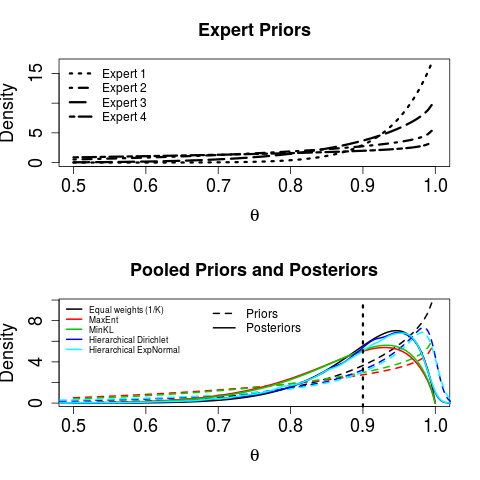
\includegraphics[width=\textwidth, height = 15cm]{figures/new_beta_example.png}
\caption{\textbf{Prior and posterior densities for $\theta$}.
Top panel shows the distributions elicited by each expert (data from~\cite{savchuk1994}) and the bottom panel shows the pooled priors and posteriors obtained using each of the three methods discussed in this paper.
The dashed vertical line marks the maximum likelihood estimate of $\theta$, $\hat{\theta}= 9/10$.
[NEEDS CHANGING]}
\label{fig:priors_posteriors_beta}
\end{figure}

\newpage 
\newpage

\section*{Appendix}

\subsection*{Proofs}

Here we provide a simple proof of theorem~\ref{thm:normalisation} using H\"{o}lder's inequality.
\begin{proof}
We begin by noting that $\pi(\theta)$ can be re-written as:
\begin{equation}
\label{eq:pirewritten}
 \pi(\theta) \propto f_0(\theta)\prod_{j=1}^{K} \left(\frac{f_j(\theta)}{f_0(\theta)}\right)^{\alpha_j}.
\end{equation}
Let $X_j = \frac{f_j(\theta)}{f_0(\theta)}, j=1, 2,\ldots, K$. 
Then integrating the expression in (\ref{eq:pirewritten}) is equivalent to finding 
\begin{equation}
\label{eq:expectations}
E_{0}\left[\prod_{j=1}^KX_j^{\alpha_j}\right] \leq \prod_{j=1}^KE_{0}[X_j]^{\alpha_j},
\end{equation}
where $E_{0}[\cdot]$ is the expectation w.r.t $f_0$ and (\ref{eq:expectations}) follows from H\"{o}lder's inequality for expectations~\citep{yeh2011}.
Since $\forall j$ we have $E_{0}[X_j]^{\alpha_j} = \left(\int_{\boldsymbol\Theta}f_0(\theta)\frac{f_j(\theta)}{f_0(\theta)}\right)^{\alpha_j}d\theta=1^{\alpha_j}=1$, Theorem~\ref{thm:normalisation} is proven.
\end{proof}
It is straightforward to show that remark~\ref{rmk:concavity} holds:
\begin{proof}
\begin{align}
 \pi(\theta) &\propto \prod_{i=0}^{K} [\exp(\psi_i(\theta))]^{\alpha_i}\\
             &\propto \exp(\psi^{\ast}(\theta)),
\end{align}
 where $\psi^{\ast}(\theta) = \sum_{i=0}^{K}\alpha_i\psi_i(\theta)$ is a concave function due to being a linear combination of concave functions.
\end{proof}
To see that equation~\ref{eq:entropypriorEF} holds:
\begin{eqnarray*} 
H_\pi(\theta) & = & E[-\log(\pi(\theta)] \\
              & = & - \int \log(\pi(\theta) \pi(\theta) d\theta \\
              & = & - \int (\log(K(a^*, b^*) + \theta a^* - \psi(\theta) b^*) \pi(\theta) d\theta \\
              & = & - \log(K(a^*, b^*) + a^*  E[\theta]-  b^*  E[\psi(\theta)]
\end{eqnarray*}
Likewise for equation~\ref{eq:KLpriorEF}, we have 
\begin{eqnarray*} 
KL(f_i || \pi) & = & E_\pi[\log(f_i(\theta)-\log(\pi(\theta)] \\
              & = & \int [\log( K(a_i,b_i) e^{\theta a_i - b_i \psi(\theta)}) - \log(K(a^*,b^*) e^{\theta a^* - b^* \psi(\theta)}) ] \pi(\theta) d\theta \\
              & = & \int [\log( K(a_i,b_i)) - \log(K(a^*,b^*)) + (a_i - a^*) \theta  - (b_i - b^*) \psi(\theta) \pi(\theta) d\theta \\
              & = & \log( K(a_i,b_i)) - \log(K(a^*,b^*)) + (a_i - a^*) E[\theta] - (b_i - b^*) E[\psi(\theta)] 
\end{eqnarray*}
\end{document} 